\chapter{Zábava a její metriky}

Pojem zábava patří mezi velice subjektivní pojmy. Pro každého je zábavného něco jiného a svět her není výjimkou. Mezi hlavní zastupitele zkoumající tento pozitivní požitek patří Mihaly Csikszentmihalyi, který ideální stav maximální zábavy, maximálního ponoření do některé z činností nazval flow. Blíže tento stav bude popsán v následující podsekci.

Přestože se jedná o pojem subjektivní, pro použití DDA je nutné najít některé složky zábavy, které jsou změřitelné, kvantifikovatelné. Musíme být schopni zábavu měřit. Jestliže ji dokážeme změřit, můžeme to využít pro stavbu DDA algoritmů a i pro měření kvalit různých algoritmů mezi sebou. Možné metriky budou popsány dále.

\section{Flow}

Flow (tok) je stav mysli, kdy je osoba v průběhu provozování činnosti naprosto soustředěná. Osoba ve stavu flow dosahuje většinou, na své poměry, nadprůměrných výkonů, ale přitom ji to nepůsobí výraznou námahu. Tento stav je většinou spojen s pocity energie, radosti, harmonie a seberealizace\cite{FlowCZ}. S pojmem Flow prvně přišel zástupce pozitivní psychologie Mihaly Csikszentmihalyi ve své práci Flow: The psychology of optimal experience, česky vydané pod názvem O štěstí a smyslu života\cite{stesti}.

Požadovaný stav lze charakterizovat z pohledu dovedností člověka a náročnosti prováděné činnosti. Dosáhneme ho, jestliže provádíme úkol náročností odpovídající našim schopnostem. Odtud pochází jeden z hlavních principů DDA, adaptivita obtížnosti hry dle schopností uživatele.

Stav flow můžeme znázornit pomocí grafu na obr. \ref{fig:ch2flow}. Jestliže se člověk seznamuje s novou činností, začíná v levém dolním rohu flow grafu. V tu chvíli nemá žádné dovednosti a pravděpodobně se začíná učit provádět činnost od jednoduchých částí po složitější. V knize \cite{OptimalFun} uvádí Csikszentmihalyi jako příklad takové činnosti hraní tenisu. Alex začíná hrát tenis, a tedy se nachází ve fázi označené $A_1$. Alex v této chvíli neumí vůbec hrát tenis a začíná s tréninkem trefování se do míčku. Není to příliš obtížné, ale Alex si to užívá, protože náročnost tohoto úkolu přesně odpovídá jeho schopnostem.

\begin{figure}
  \centering
  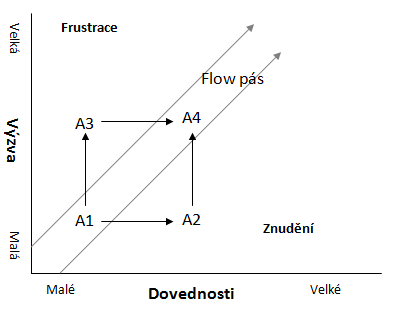
\includegraphics[width=0.5\textwidth]{ch2flow}
	\caption{Příklad pohybu jedince ve flow grafu. }
	\label{fig:ch2flow}
\end{figure}

V této chvíli se Alex pohybuje v tzv. flow pásu. Na stejném místě v diagramu nemůže zůstat Alex věčně. Jak danou činnost procvičuje, stává se v ní čím dál lepší, přestává ho to bavit, dostává se do nudy znázorněné v grafu $A_2$. V opačném případě se může stát, že potká zkušeného hráče. Hra proti němu je mnohem náročnějším úkolem a převyšuje Alexovy schopnosti. Alex se v takovém případě dostává do stavu úzkosti a stresu $A_3$.

V obou zmíněných příkladech se Alex nachází mimo flow pás a bude se snažit do něj opět dostat. V horším případě hru vzdá a další stav $A_4$ již v grafu nebude. V případě, že je ve stavu $A_2$, je dalším logickým krokem začít obtížnější úkol, vytyčit si nový cíl odpovídající jeho schopnostem. Ve stavu stresu $A_3$ má Alex jedinou možnost, zlepšit své dovednosti, aby se opět vrátil do flow pásu. Teoreticky může ubrat na výzvě, náročnosti úkolu, ale jak je jednou člověk vystaven takové výzvě, je pro něj těžké ji ignorovat a vzdát se jí\cite{OptimalFun}. 

\subsection{Flow ve hrách}

Nás bude více zajímat napojení flow na vývoj počítačových her. Jenova Chen ve své diplomové práci Flow in Games\cite{thesisflow} vybral několik flow komponent, které označil za hlavní při návrhu hry. Dle Chena musí hra obsahovat následující tři elementy, aby hráč dosáhl stavu flow.

\begin{enumerate}
	\item Předpokladem je, že hra sama o sobě je pro hráče odměňující. Hráč sám o sobě chce hru hrát.
	\item Hra nabízí správnou náročnost úkolů vzhledem k hráčovým schopnostem, což mu umožňuje více se do hry ponořit.
	\item Hráč potřebuje cítit kontrolu nad prováděnou činností.
\end{enumerate}

Jsou-li splněny všechny tři body, hráč může ztratit pojem o čase a zcela se do hry ponořit.

Stavem flow ve hrách se dále zabýval Lennart Nacket, který ve svém článku\cite{FlowAll} shrnuje spojení flow s počítačovými hrami od různých autorů. Sweetserův a Wyethův herní flow obsahuje osm složek vycházejících z 9 složek flow od M. Csikszentmihalyi (\cite{OptimalFun}, \cite{FlowEng}, \cite{FlowCZ}).

Těmito složkami jsou jasné cíle, zpětná vazba, výzva, hráčovi dovednosti, koncentrace, pocit kontroly, ponoření se do činnosti a sociální interakce.

\textit{Jasné cíle}: 
Hráč by měl být vždy schopen jasně zpracovávat herní mise, úrovně, úkoly. Aktuální úkoly by měly být vždy jednoznačné a nematoucí.

\textit{Zpětná vazba}: 
Hra by měla vždy uživatele informovat o výsledku provedených akcí. Hráč by měl být seznámen, jak se blíží, či oddaluje od splnění cíle hry.

\textit{Výzva}: 
U příliš jednoduchých her se nemohou uživatelé ponořit do hry. Hra musí být výzvou. Podstatné je rozlišovat náročnost ve formě špatně navrženého uživatelského rozhraní a ovládání a výzvu jako část herního designu. Špatné ovládání není nikdy žádoucí.

\textit{Hráčovi dovednosti}: 
Hra by měla být navržena tak, aby hráči umožňovala efektivní získávání herních dovedností. Hra by měla brát v úvahu i možné dovednosti získané hráčem z jiných her.

\textit{Koncentrace}: 
Hráč musí být do hry zcela ponořen, věnovat ji veškerou svojí pozornost.

\textit{Pocit kontroly}: 
Hráč má mít pocit, že ovládá dění ve hře. Tento bod může být kritickým u návrhu DDA. Zjistí-li hráč, že jeho úspěch ve hře není zcela závislý na jeho výkonu, ztrácí pocit kontroly.

\textit{Ponoření se do činnosti}: 
Podobné koncentraci. Hra má pohlcovat a udržovat hráče v maximální pozornosti, ale tak, aby mu to bylo stále příjemné.

\textit{Sociální interakce}: 
Tento bod je přidán oproti prvotnímu flow. K dokonalému zážitku potřebuje člověk další lidské spoluhráče a protihráče.

\subsection{Zóna flow pro různé hráče}

Vraťme se znovu ke flow diagramu na obr. \ref{fig:ch2flow}. Dle příkladu s Alexem a jeho učením se tenisu by se mohlo zdát, že pro každého je ideální udržovat zcela vyrovnanou hodnotu schopností a náročnosti úkolů a udržovat uživatele v úzkém flow pásu.

Bohužel takový flow diagram nebere v úvahu individualitu hráče. Existují zkušení hráči, kteří mají rádi větší výzvy než jsou v tu chvíli schopni zvládnout. Naopak existují příležitostní hráči, kteří netouží po velkých výzvách a nejraději se budou pohybovat lehce pod flow zónou. Těchto specifik si všímá např. práce \cite{RiskTakers}. Ideální průběh hry pro příležitostné/začínající hráče, běžné a zkušené hráče znázorňuje graf na obr. \ref{fig:ch2flowzone2}. Mnohé práce tato specifika opomíjejí a často je jejich cílem upravit obtížnost hry, aby byl vyrovnaný počet hráčových výher a proher a už neberou v potaz, že někteří hráči přestanou hrát, když budou z poloviny pokusů prohrávat.

\begin{figure}
  \centering
  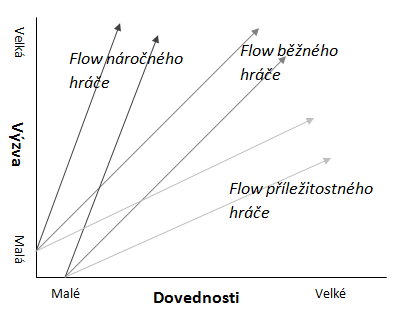
\includegraphics[width=0.5\textwidth]{ch2flowzone2}
	\caption{Flow zóna a specifika pro příležitostné a zkušené hráče. }
	\label{fig:ch2flowzone2}
\end{figure}	

\section{Metriky zábavnosti} \label{sec:defzab}

Hlavním cílem počítačových her je pobavení hráče. Z tohoto důvodu je žádoucí umět zábavu přímo, či nepřímo změřit. Pro techniku DDA je existence takové metriky zcela zásadní. Bez ní by hra nevěděla, jakým způsobem se má přizpůsobovat hráči a neuměla by ohodnotit, jestli to dělá dobře. 

Metriky můžeme rozdělit do několika kategorií. Některé metriky jsou specifické pro konkrétní hru, jiné jsou obecně použitelné pro většinu existujících her. Dále jsou metriky, jež vycházejí pouze ze stavu hry, softwaru. Protikladem mohou být speciální metriky měřící hodnoty z vnějšího světa. Příkladem může sledování srdečního tepu \cite{7}. Dále lze využít webkameru, senzory na herních i neherních zařízení. Kromě tepu lze využívat např. pevnost stisku joysticku, měnící se odpor kůže, teplotu těla\cite{16Survey}. V této práci se pro naše účely zaměřím na metriky univerzálně použitelné a získané ze stavu hry.

Zábava ve hrách se často zjednodušuje do podoby náročnosti hry vzhledem k dovednostem hráče. Z tohoto důvodu velké množství přístupů pracuje s metrikami, které zábavu měří nepřímo, měří obtížnost hry. Často používanou metrikou je hodnota win-rate, poměr vítězstvích hráče ku jeho prohrám. Hodnota 0,5 značí polovinu výher a polovinu proher. Mnohé přístupy hodnotu 0,5 berou jako ideální. V tomto případě se hra snaží obtížnosti přiblížit co nejpřesněji dovednostem hráče. Jak bylo naznačeno v předchozí sekci, ne každý hráč ocení polovinu proher. Zde je prostor pro kombinaci statické a dynamické obtížnosti. Při statické obtížnosti si hráč vybere jednu z předem daných obtížností, např. začátečník, pokročilý, expert, kterým budou odpovídat hodnoty win-rate 25, 50, 75 %.

Další metriky využívají heuristiku, která numericky ohodnotí stav hry pro každého hráče. Numerickou hodnotu nazveme ziskem. Velikost zisku nepřímo vyjadřuje pravděpodobnost výhry hráče. Samotná heuristika je herně specifická, ale prakticky u každé hry lze nějakou vymyslet, a proto jsou metriky, které ji využívají, obecně použitelné. 

Na základě této heuristiky definujeme status funkci dle algoritmu Dynamická úroveň\cite{24DynLev} a rozšíříme jí ze dvouhráčových her na jednohráčové a vícehráčové hry. U jednohráčové hry se status hráče přímo rovná jeho zisku. V ostatních případech najdeme hráče s největším ziskem. Status tohoto hráče se rovná rozdílu jeho zisku a zisku druhého hráče v pořadí. Pro ostatní hráče se status spočítá jako jejich zisk mínus zisk hráče s největším ziskem. U her s dvěma hráči bude status jednoho hráče číslo opačné ke statusu druhého hráče.

Je-li status kladný, hráč má větší šanci na výhru. V případě záporného statusu je větší pravděpodobnost hráčovy prohry. U dvou a vícehráčových her má vždy jeden hráč status kladný, ostatní mají status záporný.

Příkladem jednoduché heuristiky ve hře dáma bude počet zbývajících kamenů hráče. U hry Člověče, nezlob se může být jednoduchou heuristikou suma vzdáleností figur jednoho hráče od cíle.
 
V článku \cite{24DynLev} na základě zmíněné heuristiky přicházejí k třem metrikám. Počet změn ve vedení, napínavost během hry a konečný náskok. Všechny 4 zmíněné metriky (3 předchozí + win-rate) lze dobře využít v teorii her pro ohodnocení jednotlivých algoritmů a porovnání jich mezi sebou. 

Metriky doplníme o dalších pět nových. Počet výměn hráčů ve vedení nemusí být dostatečný. Mohlo by se stát, že každý z hráčů by byl během hry 2 krát ve vedení, ale jeden z nich by byl ve vedení 90\% času a zbylí hráči zbývajících 10\%. Z tohoto důvodu zavedeme metriku s jednoslovným názvem vedení. Další metrikou je svoboda. Hráč může ztratit zájem o hru, jestliže nemá možnosti volby a existuje-li jenom malé množství možných tahů.

Poslední 3 metriky jsou použitelné pouze u her, které jsou nedeterministické nebo které nejsou s úplnou informací. V případě neúplné informace potřebujeme, aby hra obsahovala informace, které nejsou známy ani jednomu z hráčů. Příkladem můžou být zakryté karty v balíčku, ale ne karty v soupeřově ruce. My se v rámci našeho přístupu budeme snažit náhodné jevy a neznámou informaci v rámci pravidel hry ovlivňovat, a proto se vyskytla potřeba dalších tří metrik.

Nové metriky spravedlnost a náhodnost porovnávají statusy hráčů před a po odkrytí skryté informace alespoň jednomu z hráčů (např. líznutí karty), nebo před a po projevu náhodného jevu (např. hod kostkou). Poslední metrikou je uvěřitelnost. Hra by nebyla uvěřitelná, jestliže by jednomu hráči padlo pětkrát za sebou 6, nebo pokud by si vytáhl všechny karty stejné barvy. 

Ve zbytku sekce popíši výpočet všech nastíněných metrik.

\subsection{Existující metriky}

\subsubsection{Poměr vítězství}

První metrika poměr vítězství vychází přímo z hodnoty win-rate. Hru považujeme za více zábavnou, jestliže se hráči o vítězství dělí v průběhu několika her rovnoměrně. Poměr vítězství se spočítá jako směrodatná odchylka hodnot win-rate jednotlivých hráčů.

\subsubsection{Změna vedení}

Hráč, který má kladný status, je ve vedení. Jestliže se dostane do vedení jiný hráč, zaznamená se to. Metrika měří počet výměn hráčů ve vedení během hry od začátku do konce. Je zde předpoklad, že hra je více zábavná, jestliže se hráči častěji ve vedení střídají, a tedy není pořadí hráčů stejné na začátku, během a na konci hry. 

U hry s jedním hráčem se status hráče rovná přímo jeho zisku. Metrika změna vedení u hry s jedním hráčem se rovná počtu změn znaménka statusu tohoto hráče.

\subsubsection{Náskok}

Metrika náskok je závislá pouze na aktuálním kole $a$. Udává náskok prvního hráče nad ostatními. Hodnota náskoku se přímo rovná statusu prvního hráče. Status prvního hráče v kole $a$ označíme $s^*_a$. Potom výpočet metriky lze jednoduše zapsat jako absolutní hodnotu statusu :

	\[
	naskok(a) = |s^*_a|
\]

Absolutní hodnotu můžeme vynechat u her více hráčů, kde status vedoucího hráče není nikdy záporný.

Hru budeme považovat za zábavnější, jestliže hodnota náskoku bude co nejmenší.

\subsubsection{Napínavost hry}
Napínavost je dána průměrným náskokem prvního hráče před druhým během hry od prvního do aktuálního kola a. Náskok v i-tém tahu je dán statusem hráče ve vedení, označíme jej $s^*_i$. Vzorec pro výpočet napínavosti vypadá následovně :

	\[
	napinavost(a) = \frac{1}{a}\sum_{i=1}^a{|s^*_i|}
\]

Stejně jako u náskoku, můžeme absolutní hodnotu vynechat u vícehráčových her. Opět čím nižší hodnota náskoku, tím lépe.

\subsection{Nové metriky}

\subsubsection{Vedení}

Hra nebývá příliš zábavná, jestliže po většinu času je stejný hráč ve vedení. Hra je pro všechny hráče více zábavná, jestliže se každý hráč držel přibližně stejnou dobu na prvním místě.

Metrika vedení bude udávat směrodatnou odchylku časů ve vedení jednotlivých hráčů.

Výpočet střední hodnoty vedení :
	\[
	\mu_v = \frac{1}{|P|}\sum_{p \in P} dobaVedeni(p)
\]

Výpočet metriky vedení :
	\[
	vedeni(a) = \sqrt{\frac{1}{|P|}\sum_{p \in P} |\mu_v - dobaVedeni(p)|^2}
\]

U her s jedním hráčem považujeme za dobu ve vedení počet kol, kdy hráč má kladný status. Metrika vedení se zde spočte jako směrodatná odchylka počtu kol s kladným a záporným statusem.

Opět platí, že čím menší hodnota vedení, tím považujeme hru za zábavnější.

\subsubsection{Svoboda}

Svoboda se jednoduše spočte zprůměrováním počtu možných tahů všech hráčů od začátku hry do aktuálního kola hry.

\[
	svoboda(a) = \frac{1}{a}\sum_{i=1}^a{pocetMoznychTahu_i}
\]

Čím větší hodnota svobody, tím lépe.

\subsubsection{Spravedlnost}

U nedeterministických her se nezřídka stane, že náhoda rozhodne vítěze hry. Např. u karetní hry se může stát, že i když jeden hráč hraje ideální tahy, tak přesto hru prohraje. Definujeme si spravedlnost na základě statusu všech hráčů před prvkem náhody a po něm. Rozdíl statusů před a po pro každého hráče značí, kolik a jak jsme jednotlivým hráčům pomohli, či ublížili. Hra bude nejvíce spravedlivá, jestliže všechny hráče poškodíme/pomůžeme jim stejně.

Nejdříve si spočteme pro každého hráče, jak jsme mu během hry doposud pomáhali/škodili ($s(p)$). Proměnná $\Delta status_i(p)$ značí rozdíl statusů hráče $p$ před a po náhodné události v kole $i$.

	\[
	\forall p \in P : s(p) = \frac{1}{a}\sum_{i=1}^a \Delta status_i(p)
\]

Následně metriku spravedlnosti vypočteme jako směrodatnou odchylku pro $s(p)$.

	\[
	\mu_s = \frac{1}{|P|}\sum_{p \in P} s(p)
\]

	\[
	spravedlnost(a) = \sqrt{\frac{1}{|P|}\sum_{p \in P} |\mu_s - s(p)|^2}
\]

Spravedlivější hry budeme považovat za zábavnější. Znovu platí, že čím menší hodnota metriky spravedlnosti, tím lépe.

\subsubsection{Uvěřitelnost}

Metrika uvěřitelnosti bude patřit mezi ty nejdůležitější. Dle flow musí mít hráči pocit kontroly. Jakmile získají podezření, že hra se nechová dle jejich očekávání, pocit flow se vytratí. Uvěřitelnost je silně závislá na typu hry. U každé hry je neuvěřitelné něco jiného. 

Ve hře obsahující hrací šestihranné kostky každý předpokládá, že s největší pravděpodobností každému z hráčů padne během hry každé číslo od 1 do 6 přibližně ve stejném počtu. U karetních her hráč předpokládá, že od každé barvy dostane během hry stejné množství karet. V případě, že bude dostávat pouze samé srdcové karty, přestane věřit, že hra se chová náhodně, a to i v případě, že se takto náhodný jev stal.

Přestože rozdílně vnímáme uvěřitelnost různých her, můžeme nalézt společný základní kámen pro metriku uvěřitelnosti. Definujeme si pojem uvěřitelnost pole četností.

Během hry si budeme zaznamenávat četnosti výsledků náhodných jevů. Hra bude nejvíce uvěřitelná, jestliže si budou četnosti všech jevů odpovídat. Základem uvěřitelnosti pole četností bude rozptyl četností jednoho náhodného jevu $var_1$.

Rozptyl četností hodnot je roven nule pouze v případě, že četnost všech hodnot je totožná. V případě, že suma četností všech hodnot není násobkem počtu hodnot, nemůže být rozptyl nulový, i když jev bude zcela náhodný. Po třech hodech kostkou nikdy nebude rozptyl roven nule. 

Z tohoto důvodu od $var_1$ odečteme minimální hodnotu rozptylu $var_{min}$ pro daný součet všech četností jednotlivých jevů. Minimální hodnotu rozptylu spočteme ze situace, kdy se četnosti jednotlivých jevů liší maximálně o 1. Např. po 27 hodů kostkou budou četnosti v ideálním případě 5, 5, 5, 4, 4, 4. Z těchto četností se spočte minimální hodnota rozptylu.

Nejen hry s nulovým rozdílem $var_1 - var_{min}$ jsou uvěřitelné. Z tohoto důvodu si definujeme hodnotu prahu T, při které je hra ještě stále zcela uvěřitelná. Velikost prahu je závislá na konkrétní hře. Můžeme ji určit heuristicky.

Výsledný vzorec pro uvěřitelnost pole četností :

	\[
	uveritelnostPC(a) = \left\{
  \begin{array}{l l}
    0 & \quad \text{pokud $var_1 - var_{min} \leq T$}\\
    (var_1 - var_{min}) - T & \quad \text{pokud $var_1 - var_{min} > T$}
  \end{array} \right.
\]


\subsubsection{Náhodnost}

Poslední metrikou je náhodnost/determinismus hry. U deterministických her výsledek závisí pouze na schopnostech jednotlivých hráčů. U her nedeterministických má vliv na výsledek náhoda. Budeme měřit velikost vlivu náhody. Metrika náhodnost se bude rovnat průměrnému rozdílu statusů hráčů před a po náhodném prvku ve hře. Hra bude mít nulovou náhodnost, jestliže náhodné jevy ve hře nezmění status žádného z hráčů, a tedy z hry nedeterministické vznikne hra deterministická.

	\[
	nahodnost(a) = \frac{1}{a |P|}\sum_{i=1}^a{\sum_{p \in P} |\Delta status_i(p)|}
\]

Narozdíl od ostatních metrik zde nelze říct, že hry s menší hodnotou náhodnosti jsou zábavnější. Vnímání vlivu této metriky bude subjektivní.
